\section{Characterizing weakly-coupled carbon spins}
Using the knowledge about the interaction between the NV-center and individual nuclear spins it is possible to implement basic gates and characterize the spins.
This section will explain how basic gates can be implemented and use these gates to measure the precession frequency and $T_2&*$ of individual carbon spins.

\subsection{Basic operations}
In order to implement basic gates on a nuclear spin we make use of the conditional rotation that occurs on the resonance given by \cref{eq:res_dip_loc}.
At the resonant condition the nuclear spin rotates about one of two anti-parallel axes depending on the electronic-spin state.
The angle of the rotation is proportional to $N$.



It is possible to calibrate the angle of rotation by bringing the electronic-spin in a superposition, sweeping $N$ and measuring the contrast.
If the contrast is sweeped to -1 an unconditional $\pi$-pulse is implemented, being able to sweep the contrast to -1 means the spin is controllable.

By choosing $N$ at 0 contrast on such a spin a conditional $\pi/2$ rotation is implemented.
The rotation rotates in the clockwise direction when the electron is in the $\ket{0}$-state and in the counterclockwise direction when it is in the $\ket{1}$-state.
We define the axis of rotation of this operation as the $x$-axis and call the operation the $\pm \mathrm{x}$-gate.

The $\pm\mathrm{x}$-gate forms the basis of our control over weakly coupled spins.
\Cref{fig:gate_circuit_pm-x} shows how the $\pm \mathrm{x}$-gate is depicted in a circuit-diagram.
An unconditional gate can be implemented by placing the electron in an eigenstate before performing the $\pm\mathrm{x}$-operation.
Van der Sar et al. \citep{Sar2012DecoherenceProtected} have demonstrated how to integrate regular operations on the NV-spin with a decoupling sequence.
By letting the phase of the carbon evolve we are able to apply operations on the carbon-spin with arbitrary phase.


\begin{figure}[htbp]
    \centering
        \mbox{
        \Qcircuit @C=1em @R=.7em {
         \lstick{\ket{\Psi}_e} &\ctrl{1}  &\qw\\
          \lstick{\ket{\Psi}_\mathrm{C}} &\gate{\pm \mathrm{x} }  &\qw}}
    \caption{The $\pm\mathrm{x}$-gate performs an x-rotation on the carbon ($\ket{\Psi}_\mathrm{C}$) when the electron is in the $\ket{0}_e$-state. It performs a $-\mathrm{x}$ rotation when the electron is in the $\ket{1}_e$-state.}
    \label{fig:gate_circuit_pm-x}
\end{figure}

The $\pm\mathrm{x}$-gate has been calibrated for several spins.
The parameters used to implement $\pm\mathrm{x}$-gates are listed in \cref{tbl:gate_parameters}.
Carbon-1 and carbon-4 were found to perform the best $\pm\mathrm{x}$-gates.

\begin{table}[htbp]
    \centering
    \begin{tabular}{cccc}
    Carbon &  $ N $ &  $\tau$ & total gate time\\ \hline
    1 &  18 & { }9.420 $\mu$s & 339 $\mu$s \\
    2 & 26 & { }6.620 $\mu$s & 344 $\mu$s \\
    3 & 14 & 18.564 $\mu$s & 520 $\mu$s \\
    4 &  40 & { }6.456 $\mu$s & 516 $\mu$s
    \end{tabular}
    \caption{Parameters used to implement $\pm\mathrm{x}$-gates.}
    \label{tbl:gate_parameters}
\end{table}



\subsection{Carbon Ramsey experiment }
By performing a Ramsey experiment the precession and dephasing-time $T_2^*$ can be determined.
By determining the precession frequencies it is possible to track phase evolution and use it to implement operations with arbitrary phase.
By measuring the precession frequency it is also possible to disprove our estimation for the hyperfine parameters.
The dephasing time must be measured to determine if it is long enough to implement the gates required for QEC.

In an ordinary Ramsey experiment a qubit is brought to the equator of the Bloch-sphere where it precesses for a time $\tau $ before it is read out along the x-direction.
A carbon-Ramsey experiment is similar but slightly more complicated as the nuclear spin cannot be controlled and read-out directly.
\begin{figure}[htbp]
        \centering
        \mbox{
        \Qcircuit @C=1em @R=.7em {
        \lstick{\ket{0}}          & \gate{\mathrm{y}}  & \ctrl{1}      & \qw & \multigate{1}{T}       &  \qw &\ctrl{1}          & \gate{\mathrm{-y}}  &  \meter \\
        \lstick{\rho_\mathrm{m}}         & \qw              &  \gate{\pm \mathrm{x}}     & \qw& \ghost{T}        & \qw & \gate{\pm \mathrm{x}}      & \qw       &\qw&}}
    \caption{Gate circuit depicting an uninitialized carbon Ramsey. $T$ is the free evolution time.}
    \label{fig:gate_circuit_nuclear_ramsey}
\end{figure}

A gate circuit of the uninitialized carbon-Ramsey experiment is depicted in \cref{fig:gate_circuit_nuclear_ramsey}.
The first pulse brings the electronic spin in the $\ket{X}$-state.
Because the carbon starts out in a mixed state the two-qubit system can be described by the tensor product of two density matrices:
\begin{equation}
    \rho_X \otimes \rho_m = \rho_X \otimes \rho_{X} +\rho_X \otimes \rho_{-X}
\end{equation}
By applying the $\pm{\mathrm{x}}$-gate  the electronic-spin picks up a phase depending on the nuclear spin-state:
\begin{equation}
     \rho_Y \otimes \rho_{X} +\rho_{-Y} \otimes \rho_{-X}
    \label{eq:density_after_Ren}
\end{equation}
In this state it is left to freely evolve for a time $T$.
The last part of the uninitialized carbon-Ramsey reads out along the $x$-direction for $\ket{Y}_e$ and along the $-x$-direction for $\ket{-Y}_e$.
The phase picked up during free evolution show up as an oscillation between $\ket{0}_e$ and $\ket{1}_e$ in the readout.

\subsubsection{Determining the precession frequency}
Because the uninitialized carbon-Ramsey evolves with two frequencies we expect the measured oscillation to be the sum of two cosines as described by \cref{eq:carbon_ramsey_expected}. Where $ \tilde\omega =   \sqrt{(\omega_L+A_\parallel) ^2 + A_\perp^2} $.

\begin{equation}
    \tfrac{1}{4} \cos(\omega_L \tau ) +\tfrac{1}{4}  \cos (\tilde{\omega} \tau ) + \tfrac{1}{2}
    \label{eq:carbon_ramsey_expected}
\end{equation}

\begin{figure}[htbp]
    \begin{subfigure}[t]{0.49\textwidth}\centering
        \caption{}
        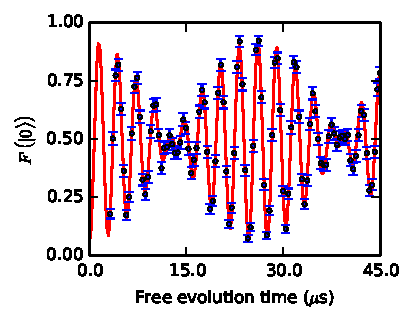
\includegraphics{Img/CarbonRamsey_C1.pdf}
        \label{fig:CR_C1}
    \end{subfigure}
    \begin{subfigure}[t]{0.49\textwidth}\centering
        \caption{}
        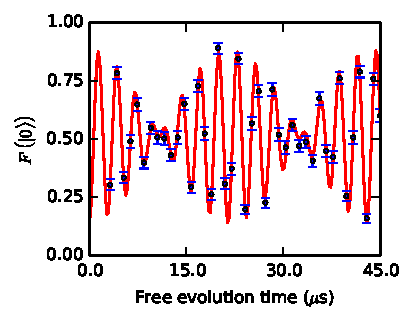
\includegraphics{Img/CarbonRamsey_C4.pdf}
        \label{fig:CR_C4}
    \end{subfigure}
    \caption{The uninitialized carbon-Ramsey experiment shows an oscillation due to the phase picked up during free evolution.
    \Cref{fig:CR_C1} shows data for carbon-1 and \Cref{fig:CR_C4} for carbon-4.
    The measured frequencies were, for carbon-1: $\omega_{L,C1} = 2\pi\cdot 325.81 \pm 0.25$ and  $\tilde \omega_{\mathrm{C1}}= 2\pi\cdot 364.41 \pm 0.23$, and for carbon-4: $\omega_{L,C4} =  2\pi\cdot 325.94 \pm 0.40$ and $\tilde \omega_{\mathrm{C4}} = 2\pi\cdot 371.52 \pm 0.39 $.}
    \label{fig:Uninitialized_carbon_ramsey}
\end{figure}

\Cref{fig:Uninitialized_carbon_ramsey} shows the results for an uninitialized carbon-Ramsey experiment.
The data was fitted to a sum of two cosines in order to determine the frequencies.

The Larmor frequencies measured are $\omega_{L,C1} = 2\pi\cdot 325.81 \pm 0.25$kHz  for carbon-1 and  $\omega_{L,C4} =  2\pi\cdot 325.94 \pm 0.40$kHz for carbon-4.
Both the measured Larmor frequencies agree with the magnetic field of 304G within two standard deviations.

The $\tilde{\omega}$ frequency can be used to disprove the estimations for the hyperfine parameters listed in \cref{tbl:HF_par}, however if the measured values agree with the hyperfine estimation we cannot conclude that the estimations are correct.

Based on the estimated hyperfine parameters we expect $\tilde\omega_{\mathrm{C1}} \approx 2\pi\cdot 364.7\mathrm{kHz}$ for carbon-1 and $\tilde \omega_{\mathrm{C4}} \approx 2\pi\cdot 371.4 \mathrm{kHz}$ for carbon-4.
For carbon-1 $\tilde \omega_{\mathrm{C1}}= 2\pi\cdot 364.41 \pm 0.23$kHz was measured
and for carbon-4 $\tilde \omega_{\mathrm{C4}} = 2\pi\cdot 371.52 \pm 0.39 $kHz was measured.
Both these values are in good agreement with experiment, an indication that our hyperfine estimation is accurate.


\subsubsection{Measuring $T_{2,\mathrm{C}}^* $}
% Lange carbon ramseys van Hans sil01 140506 #53 en 56 +T2* analyse.
% hoeveel pulses voor de lange tau? belangrijk voor T2*
To determine $T_{2,\mathrm{C}}^* $ for normal operation an uninitialized carbon-Ramsey was performed where the electron was dynamically-decoupled during the free evolution time.
Because the electron is constantly flipped the carbon will precess with an average frequency of $\omega_{\mathrm{DD}} = (\omega_L +\tilde{\omega} )/2$.
By undersampling with a frequency slightly detuned from the precession frequency ($\omega_{\mathrm{DD}}$) a decaying cosine can be observed where the 1/e time of the envelope is equal to $T_2^*$. \footnote{This note will be removed: I want to make the statement about using this method to determine frequencies: Because the experiment extends for a long time the detuning to the precession frequency can be very accurately determined making this method also useful for determining frequencies.}

\begin{figure}[htbp]
    \begin{subfigure}[t]{0.49\textwidth}\centering
        \caption{}
        \includegraphics{Img/Carbon1_T2star.pdf}
        \label{fig:T2star_carbon1}
    \end{subfigure}
    \begin{subfigure}[t]{0.49\textwidth}\centering
        \caption{}
        \includegraphics{Img/Carbon4_T2star.pdf}
        \label{fig:T2star_carbon4}
    \end{subfigure}
    \caption{Carbon-Ramsey experiment to determine $T_2^*$ for nuclei while decoupling the electron.
    The decays are fitted with a generalized normal distribution to determine $T_2^*$ and the exponent $n$.
    \Cref{fig:T2star_carbon1}, for carbon-1, $T_{2,\mathrm{C1}}^* =9.85 \pm   0.39 \mathrm{ms}$ and $n= 1.83 \pm 0.19$.
    \Cref{fig:T2star_carbon4}, for carbon-4,  $T_{2,\mathrm{C4}}^* =6.68 \pm   0.22 \mathrm{ms}$ and $n= 2.31 \pm 0.31$. } %would like to add that not limited by electron coherence due to DD.
    \label{fig:T2star_carbon}
\end{figure}

\Cref{fig:T2star_carbon} shows the decay for both carbons.
The decay follows a Gaussian profile within uncertainty for both spins.
The coherence times measured were $T_{2,\mathrm{C1}}^* =9.85 \pm   0.39 \mathrm{ms}$ for carbon-1 and $T_{2,\mathrm{C4}}^* =6.68 \pm   0.22 \mathrm{ms}$ for carbon-4.
It should be noted that these $T_2^*$ values are not limited by the electron coherence.


